\documentclass{article}
\usepackage[utf8]{inputenc}
\usepackage[margin=0.675in]{geometry}
\usepackage{amsmath}
\usepackage{graphicx}
\usepackage{float}
\usepackage{hyperref}
\usepackage{listings}

\graphicspath{{images/}}
\title{Report for Lab-Tutorial : CS3543 - Computer Networks - 2}
\author{Vishwak Srinivasan\\
\texttt{CS15BTECH11043}}
\date{}

\begin{document}
\maketitle 

\section{Transport Layer capturing}
\subsection{Capturing during Internet Download}
\begin{flushleft}
For this capture, I downloaded the \href{http://releases.ubuntu.com/17.10/ubuntu-17.10.1-desktop-amd64.iso}{Ubuntu 17.10 image file}. The duration of the capture was 240 seconds (as opposed to the suggested 60 sec), since the bandwidth was high and there were not a lot of duplicate ACKs being generated. I also used Wireshark on Windows, since I faced issues with Ubuntu's network manager.
\end{flushleft}

\subsubsection{Plot of Round Trip Time (RTT) versus wall-clock time for 240 seconds}
\begin{flushleft}
This graph was obtained using a graphing tool in Wireshark. You need to go to \texttt{Statistics --> TCP Stream Graphs --> Round Trip Time}, also shown in the picture below:
\begin{figure}[H]
\centering
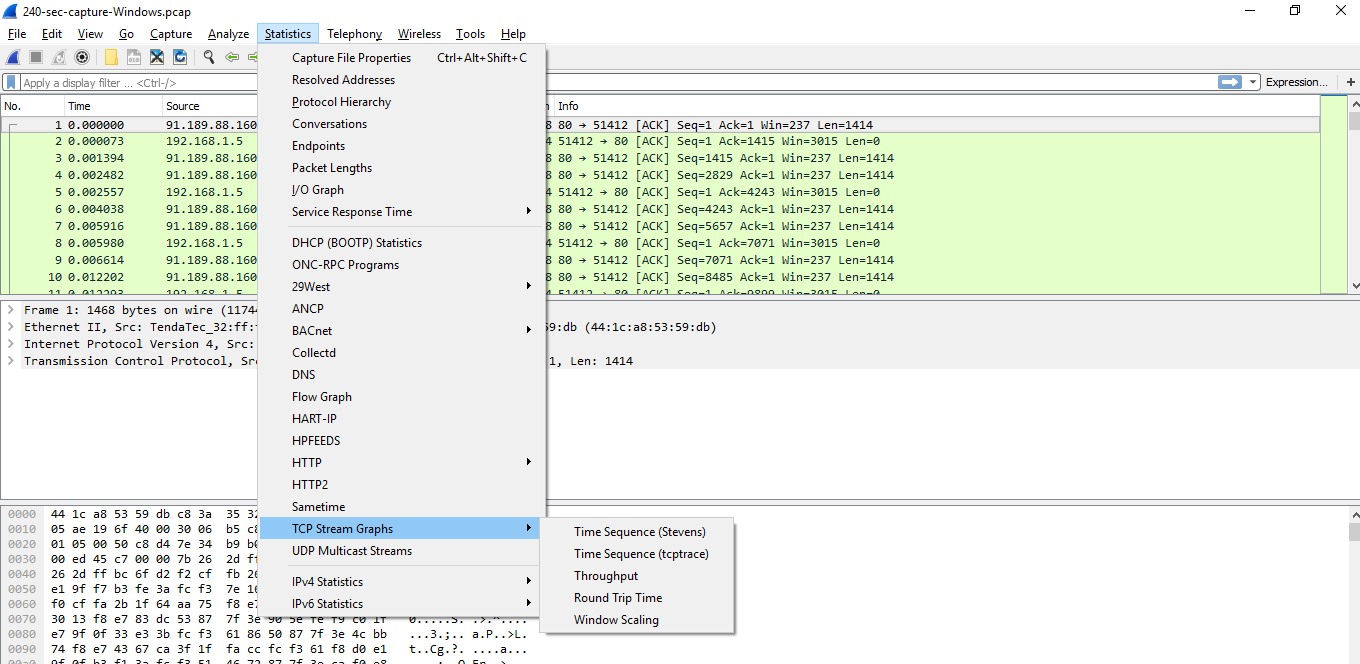
\includegraphics[width=0.6\linewidth]{RTT-Window-size-capture-process.png}
\end{figure}

The plot is shown below. The RTT values seem consistent between 0 - 8 milli-seconds, with certain outliers. Observing the \texttt{PCAP} file revealed that these outliers generally occurred in parallel with when the window size was higher.
\begin{figure}[H]
\centering
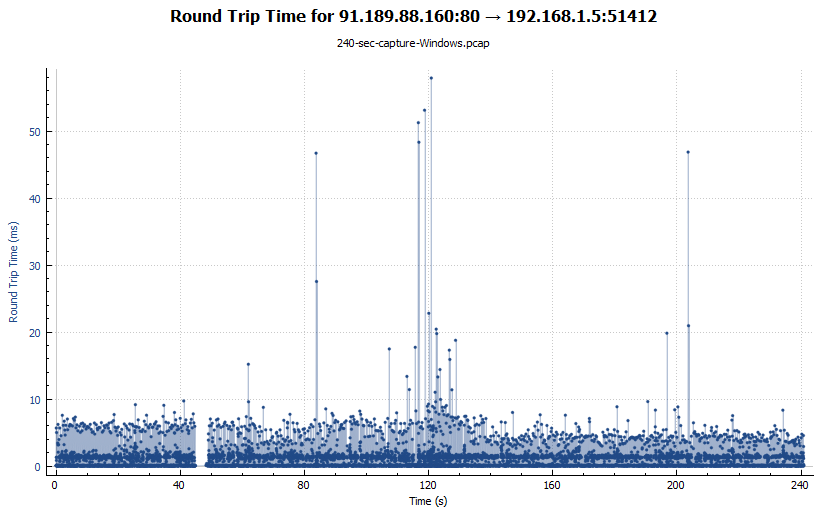
\includegraphics[width=0.65\linewidth]{RTT-variation-240-sec-capture-Windows-time.png}
\end{figure}
\end{flushleft}

\subsubsection{TCP Congestion Window}
\begin{flushleft}
I have plotted the variation of \texttt{tcp.analysis.bytes\_in\_flight} versus wall-clock time. This provides a reasonable estimate of the TCP congestion window, since this information is actually not advertised.
\begin{figure}[H]
\centering
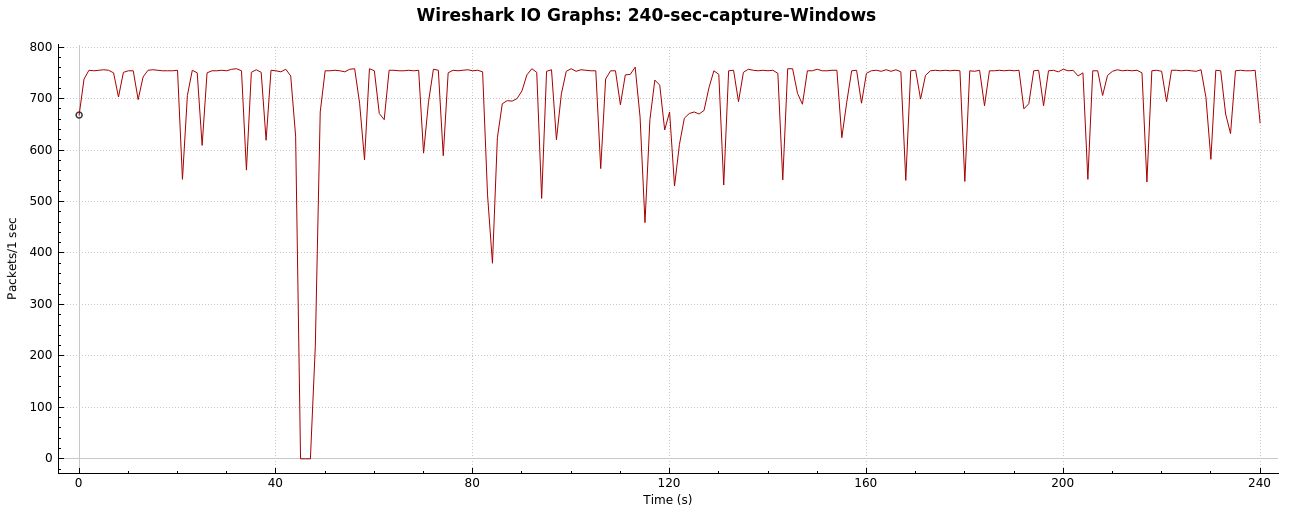
\includegraphics[width=0.75\linewidth]{tcp-CWND.png}
\end{figure}
\end{flushleft}

\subsubsection{Flow Graph}
\begin{flushleft}
Owing the large number of the packets that were captured, the entire flow graph is hard to see in this document, let alone on a 8 GB machine. Below are some snapshots taken despite the lag:
\begin{figure}[H]
\centering
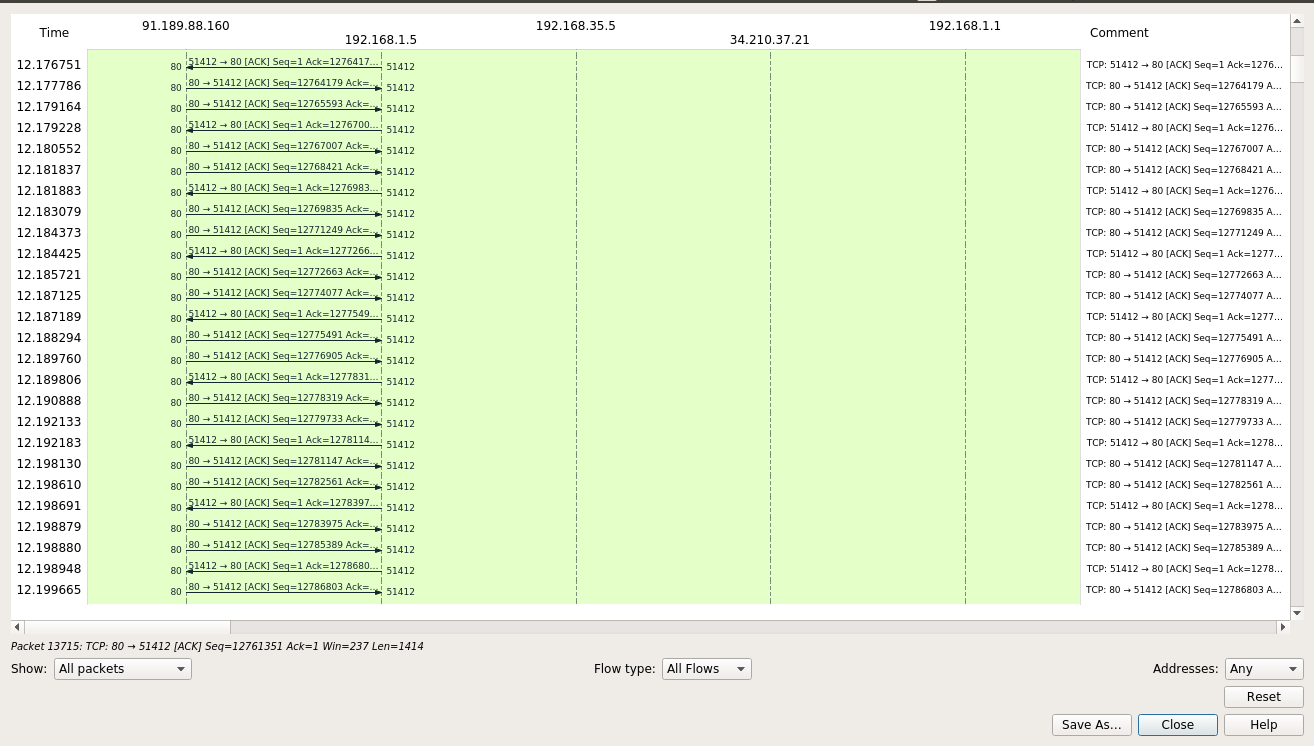
\includegraphics[width=0.6\linewidth]{flow-graph-1.png}
\end{figure}
\begin{figure}[H]
\centering
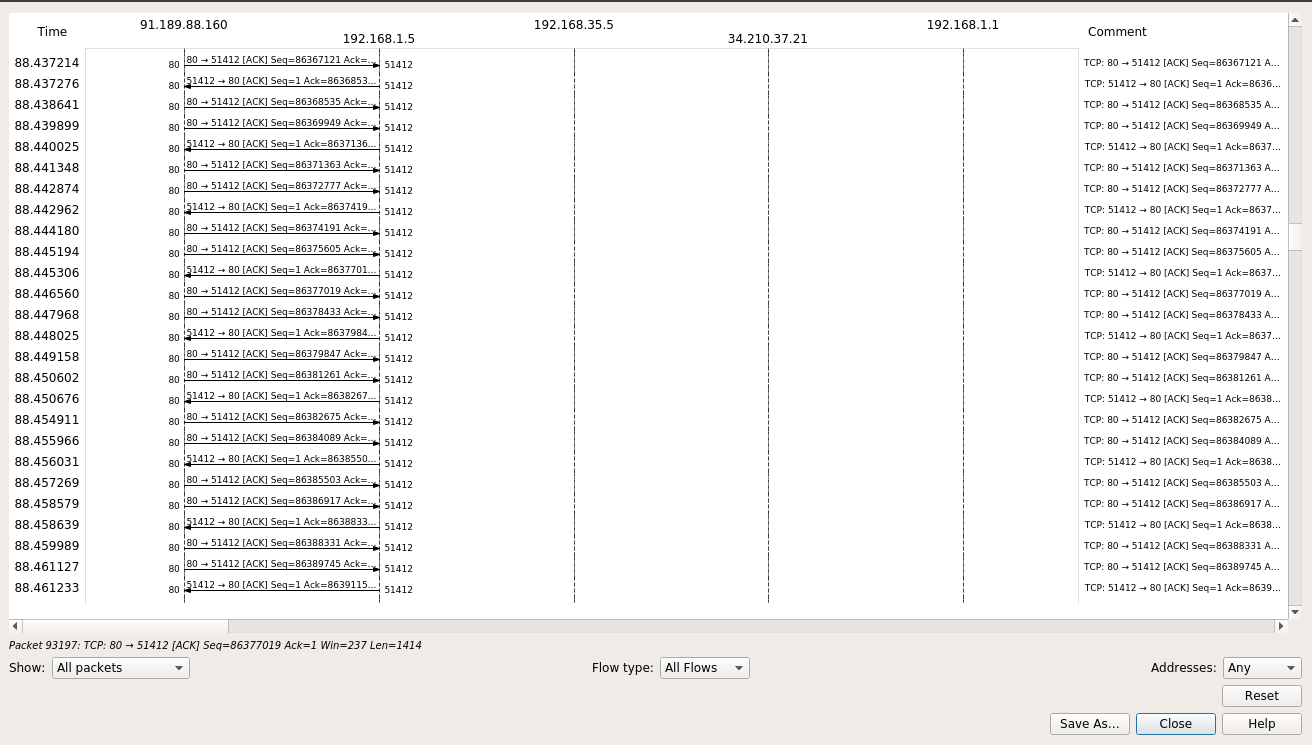
\includegraphics[width=0.6\linewidth]{flow-graph-2.png}
\end{figure}
\end{flushleft}

\subsubsection{Average Throughput and variation of throughput with wall-clock time}
\begin{flushleft}
This graph was again obtained using a graphing tool in Wireshark, available at \texttt{Statistics --> TCP Stream Graphs --> Throughput}. Here the graph is plotted with a moving average over 1 second, and is shown below:
\begin{figure}[H]
\centering
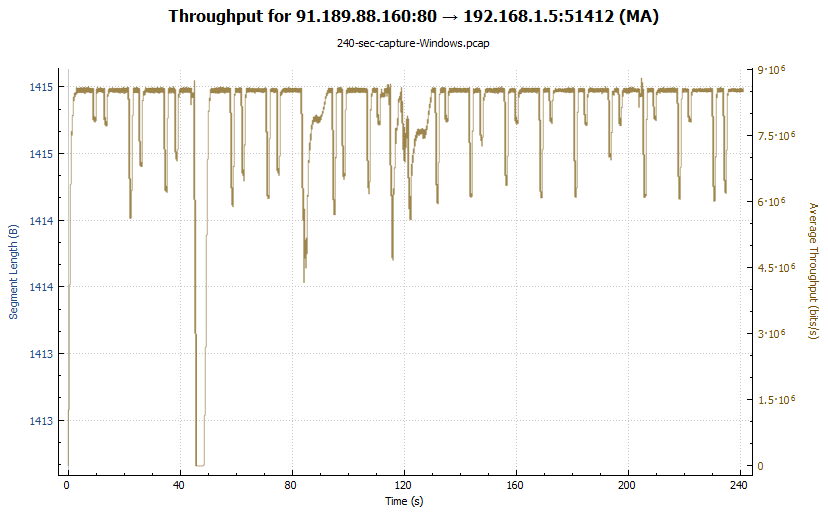
\includegraphics[width=0.55\linewidth]{Throughput-variation-240-sec-capture-Windows.png}
\end{figure}

The average throughput is \(\frac{256254658 \text{ Bytes}}{240.865 \text{ seconds}} \approx \) \boxed{1063893.29 \text{ Bps}} or \boxed{1063.89 \text{ KBps}}. This was obtained through \texttt{Capture File Properties}, and the required image is displayed below:
\begin{figure}[H]
\centering
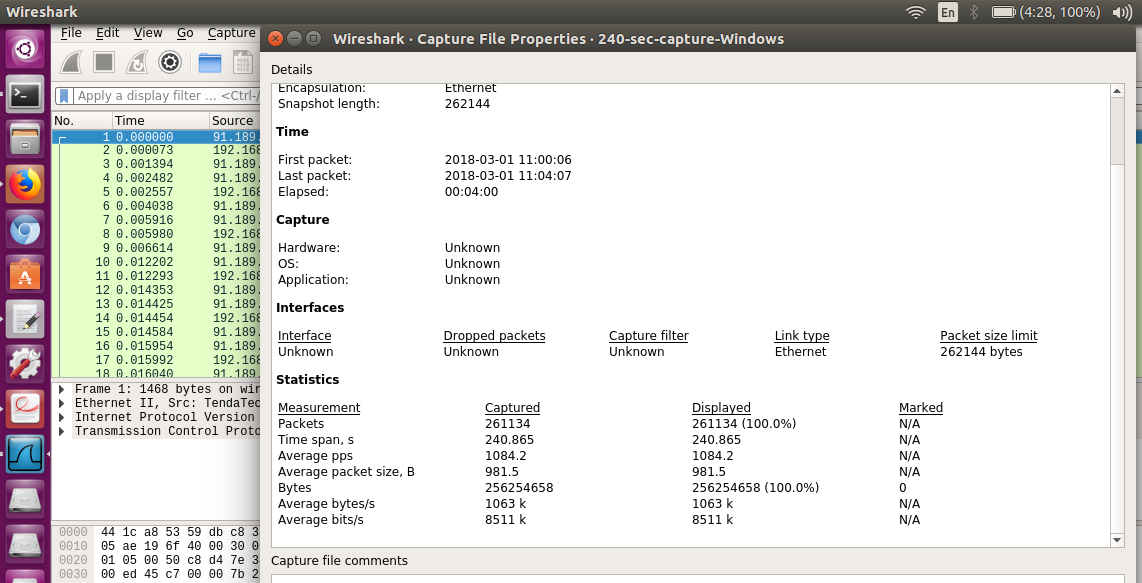
\includegraphics[width=0.55\linewidth]{Packet-capture-stats-240-sec-capture-Windows.png}
\end{figure}
\end{flushleft}

\subsubsection{Receiver Congestion Window size variation with wall-clock time}
\begin{flushleft}
This graph plots the size of the Congestion Window Size (\texttt{cwnd}), using the same Wireshark graphing tool. Here you can observe that the when window size is higher, the RTT is also higher as shown in the other graph. Eventually, a high window size causes a delay, which is when the window size decreases. This variation is graphically represented below:
\begin{figure}[H]
\centering
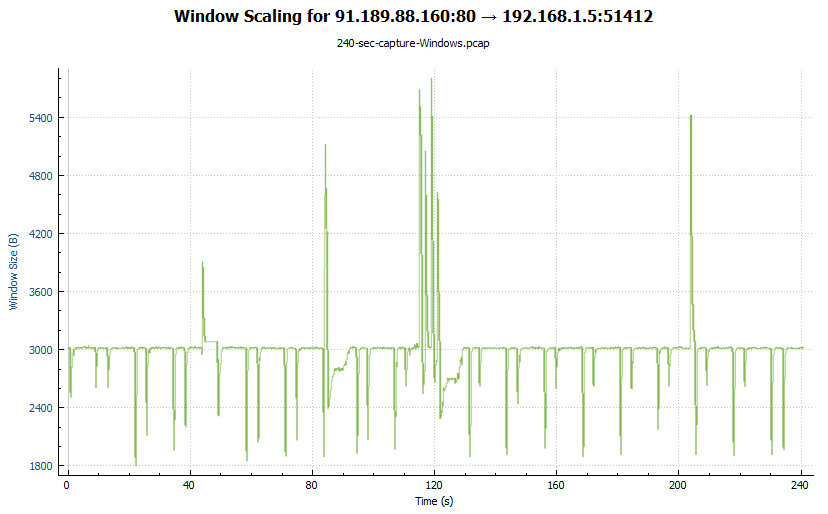
\includegraphics[width=0.55\linewidth]{Window-size-variation-240-sec-capture-Windows.png}
\end{figure}
\end{flushleft}

\subsubsection{Number of 1-DupACK, 2-DupACK and 3-DupACK with wall-clock time}
\begin{flushleft}
This can be extracted using the filter \texttt{tcp.analysis.duplicate\_ack\_num == <number>}, where \texttt{number} is either 1, 2 or 3 in this case. The filters need to be added to the IO Graph to view the variation graphically, and the process is shown below:
\begin{figure}[H]
\centering
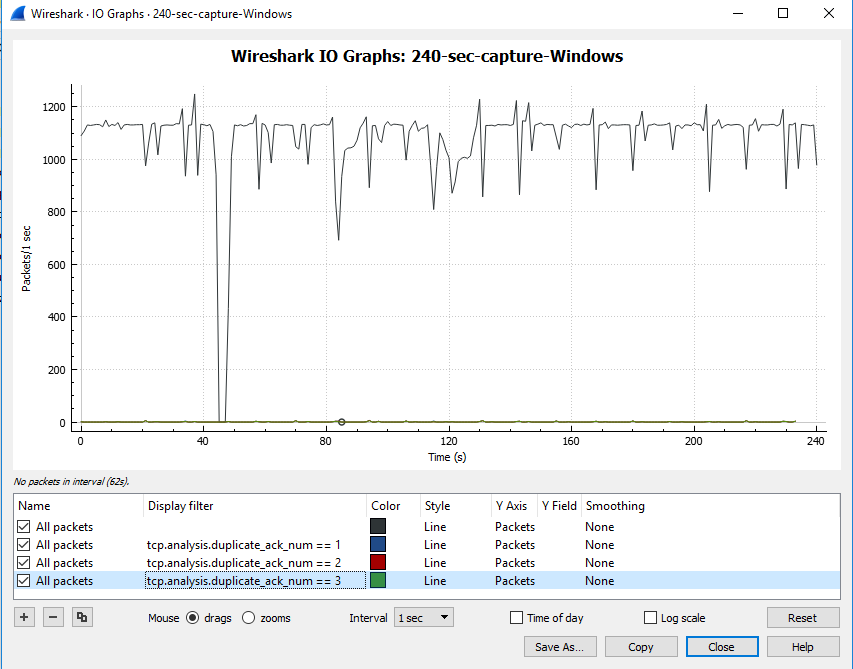
\includegraphics[width=0.55\linewidth]{dup-ack-capture-process.png}
\end{figure}

The variation in the number of 1-DupACK, 2-DupACK and 3-DupACK is shown below (top-left: 1-DupACK, top-right: 2-DupACK and bottom-center: 3-DupACK).
\begin{figure}[H]
\begin{minipage}{0.48\linewidth}
\centering
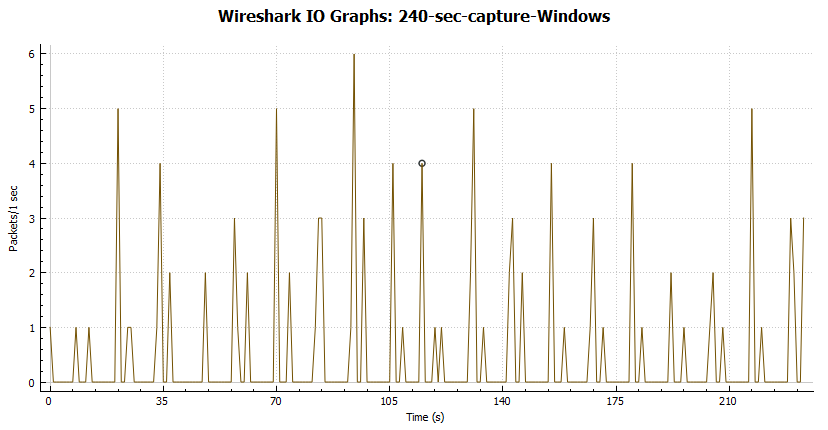
\includegraphics[width=0.975\textwidth]{1-dup-ack.png}
\end{minipage}
\hfill
\begin{minipage}{0.48\linewidth}
\centering
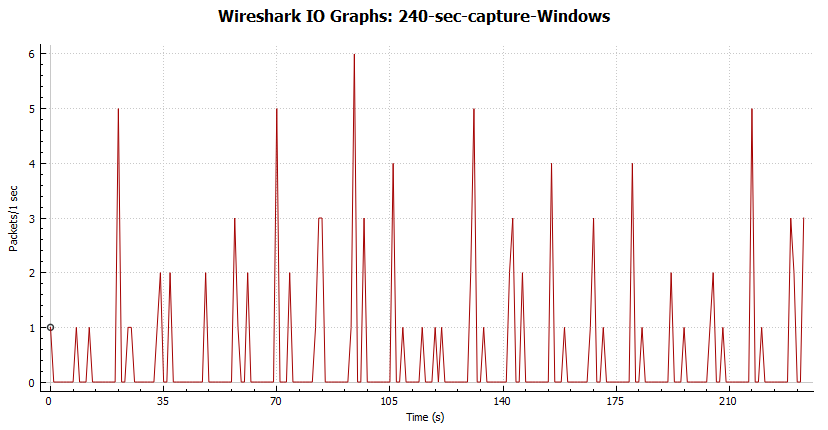
\includegraphics[width=0.975\textwidth]{2-dup-ack.png}
\end{minipage}
\end{figure}
\begin{figure}[H]
\centering
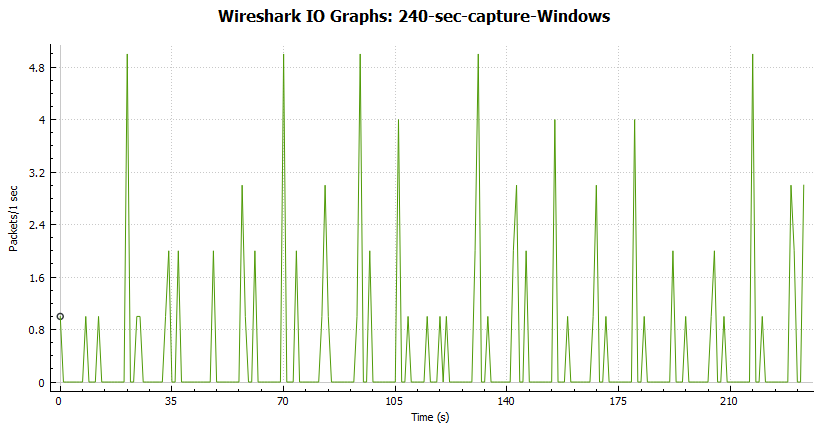
\includegraphics[width=0.47\textwidth]{3-dup-ack.png}
\end{figure}

Infact, I could observe larger number of duplicate ACKs for a packet (order of 20). I suspect the cause of this to be a passive connection gone active (Apple devices tend to do this) to the router, which caused a bottleneck in the instantaneous bandwidth for the laptop on which this was being captured.
\end{flushleft}

\subsection{Identifying the TCP 3-way handshake}
\begin{flushleft}
I downloaded a file from \href{http://unec.edu.az/application/uploads/2014/12/pdf-sample.pdf}{this link} to test this. To synchronize the download initiation and the packet capturing, I used Windows \texttt{timeout} command as a countdown for both and captured subsequently. The TCP 3-way handshake could be seen at the beginning, after which the packets began getting transmitted from the server to the client. The handshake as observed in the \texttt{PCAP} file is shown below:
\begin{figure}[H]
\centering
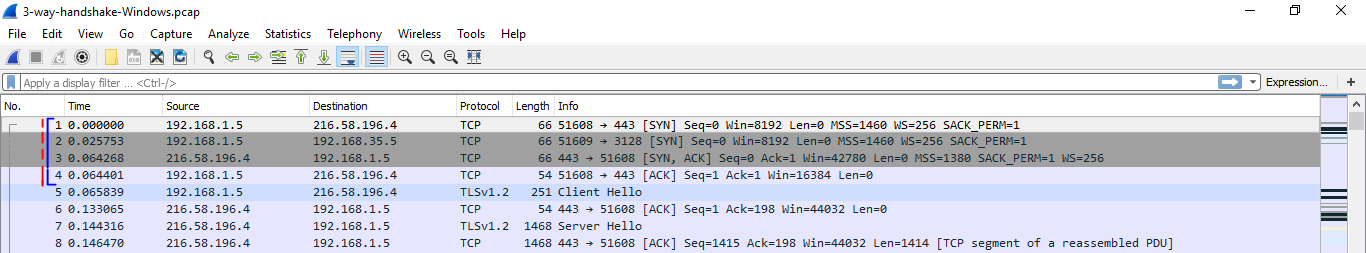
\includegraphics[width=\linewidth]{3-way-handshake-identify.png}
\end{figure}

Note the \texttt{SYN} and \texttt{ACK} being transmitted across hosts, as done in the 3-way handshake.
\end{flushleft}

\subsection{Ping and Capture}
\begin{flushleft}
It is known that a ping generates a \texttt{ICMP} packet. Since this was done with Windows, I used \texttt{timeout} to try and start the \texttt{ping} and capture simultaneously. The number of ping was 20. Below is a snapshot from Wireshark during the capture:
\begin{figure}[H]
\centering
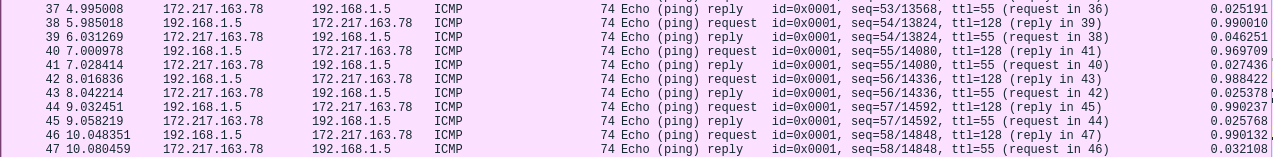
\includegraphics[width=\linewidth]{ping-snapshot.png}
\end{figure}

As learned, the type of the packet is an ICMP packet. One can note more control information sent with the packet as well.
\end{flushleft}

\subsection{Ping and Capture - with \texttt{nmap}}
\begin{flushleft}
I used \texttt{nmap} on Windows after downloading it from their \href{http://nmap.org}{site}. Using \texttt{nmap -PS} and the IP of \url{https://google.com} which I resolved the IP for, I was able to capture the types of packets sent. These packets were not \texttt{ICMP} packets - they are infact \texttt{SYN} and \texttt{ACK} packets, which means that they perform a TCP 3-way handshake with the host. Below is a snapshot of one such handshake performed during the capture:
\begin{figure}[H]
\centering
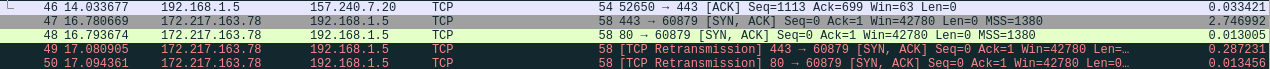
\includegraphics[width=\linewidth]{nmap-snapshot.png}
\end{figure}

Reading more about \texttt{nmap}, I found out that \texttt{nmap -PS} basically mean \emph{port scanning}, where a 3-way handshake is performed, and the connection is immediately terminated to avoid a DoS attack.
\end{flushleft}
\newpage

\section{Link Layer capturing}
\begin{flushleft}
Below is the protocol hierarchy using which some of the information for the next few questions were obtained:
\begin{figure}[H]
\centering
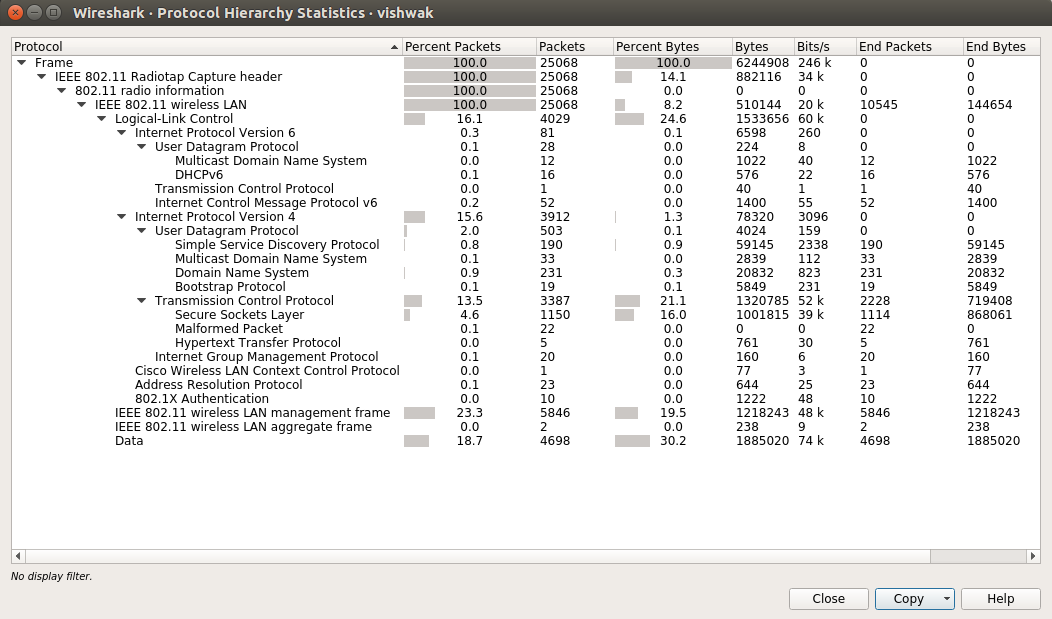
\includegraphics[width=0.7\linewidth]{protocol-hierarchy.png}
\end{figure}
\end{flushleft}
\subsection{Packet classification: Control, Data and Management}
\begin{flushleft}
Approximately 25000 packets were captured over Wi-Fi with multiple hosts in the network. Below are the counts and fractions:
\begin{center}
\begin{tabular}{|c|c|c|}
\hline
Class & Number of Packets & Fraction of Packets \\
\hline
\hline
Control & 4029 & 0.161 \\
\hline
Data & 4698 & 0.187 \\
\hline
Management & 5846 & 0.233 \\
\hline
\end{tabular}
\end{center}
\end{flushleft}

\subsection{Packet types: \texttt{ARP}, Broadcast, \texttt{TCP}, \texttt{UDP}, \texttt{ICMP(v6)} and \texttt{IGMP}}
\begin{flushleft}
Below are the counts and fractions for the different types:
\begin{center}
\begin{tabular}{|c|c|c|}
\hline
Type & Number of Packets & Fraction of Packets \\
\hline
\hline
\texttt{ARP} & 23 & 0.0009 \\
\hline
Broadcast & 5187 & 0.207 \\
\hline
\texttt{TCP} & 3390 & 0.135 \\
\hline
\texttt{UDP} & 531 & 0.0212 \\
\hline
\texttt{ICMP(v6)} & 52 & 0.0021 \\
\hline
\texttt{IGMP} & 20 & 0.0008 \\
\hline
\end{tabular}
\end{center}
Broadcast message were filtered using the filter \texttt{wlan.da == ff:ff:ff:ff:ff:ff}.
\end{flushleft}

\subsection{Unique users using MAC addresses}
\begin{flushleft}
For this, I had to add two new fields \texttt{Dest-MAC} and \texttt{Src-MAC}, and had to export it to a CSV. From there, I used Pandas, a Python library to extract the distinct MAC addresses which were both destination and source. There were 19 of them, which is displayed below:
\begin{figure}[H]
\centering
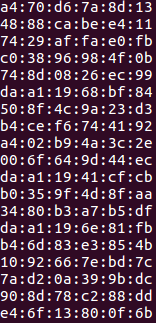
\includegraphics[width=0.25\linewidth]{users-mac.png}
\end{figure}
The source code is:
\begin{lstlisting}[basicstyle=\footnotesize\ttfamily, showstringspaces=false, language=Python]
import pandas as pd
data = pd.read_csv(`MAC-dest-src.csv', sep=`,', usecols=[`Dest-MAC', `Src-MAC'])
u_set = set(data[`Dest-MAC'].tolist()) & set(data[`Src-MAC'].tolist())
print("\n".join(list(u_set)[1:]))
\end{lstlisting}
\end{flushleft}

\subsection{Traffic Pattern}
\begin{flushleft}
This was done using IO graph, which revealed the packet variation with wall-clock time:
\begin{figure}[H]
\centering
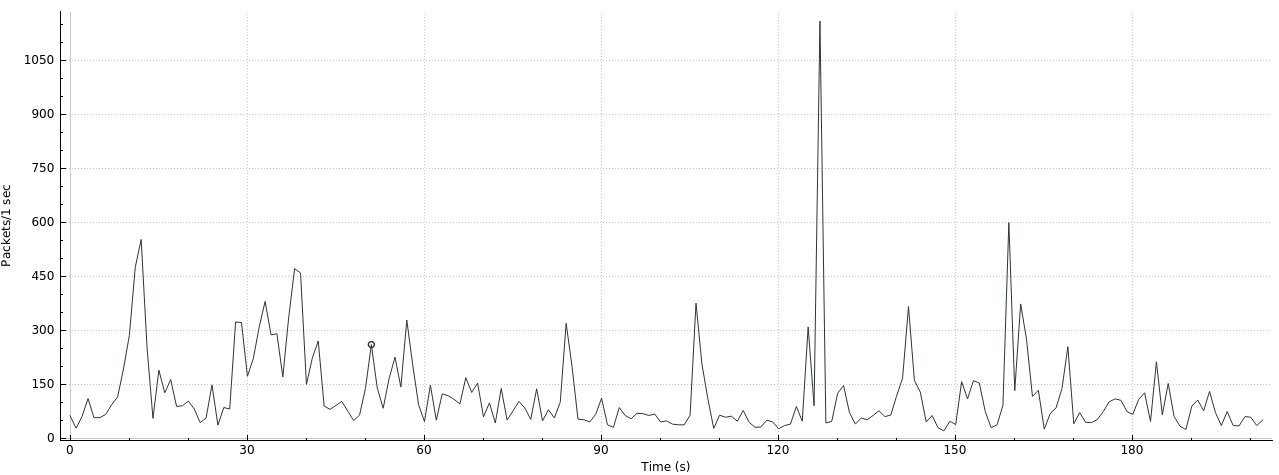
\includegraphics[width=0.75\linewidth]{traffic-pattern-l2.png}
\end{figure}
\end{flushleft}

\subsection{Number of ``special" retransmission}
\begin{flushleft}
The number of these retransmissions not accompanied by a link-layer ACK can be found using the filter \texttt{wlan.lc.retry eq 1}. Out of around 25000 frames, 1329 frames where ``specially" retransmitted. Below is the snapshot:
\begin{figure}[H]
\centering
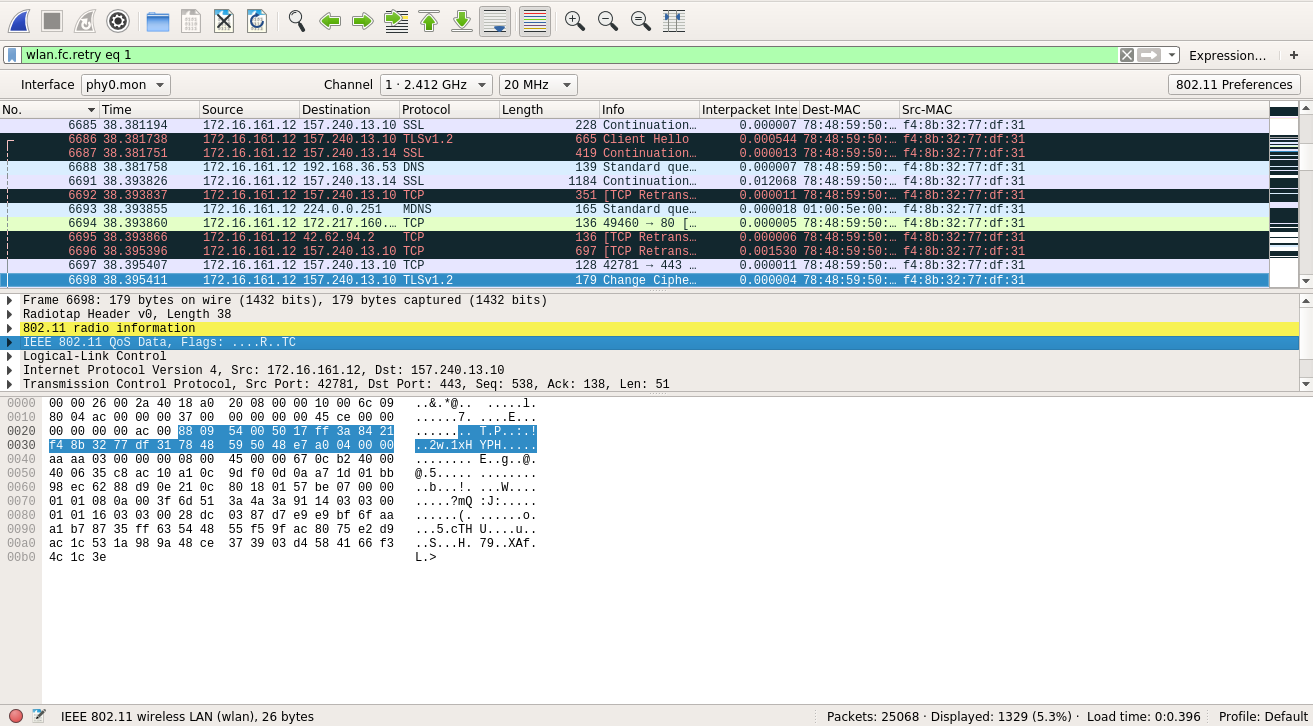
\includegraphics[width=0.85\linewidth]{snapshot-retrans.png}
\end{figure}
\end{flushleft}
\end{document}
